%!TeX root=../document.tex

\chapter{Dynamic Solution}

The equation of motion of the system takes the form of a second-order ordinary differential equation (ODE).
Together with the initial displacements~$\boldsymbol{u}_0$ and velocities~$\mathbf{v}_0$ at time $t_0$ they form the second-order initial value problem
%
\begin{align}
&\boldsymbol{M}\ddot{\boldsymbol{u}} + \boldsymbol{Q}(\boldsymbol{u},\,\dot{\boldsymbol{u}}) = \boldsymbol{P}(t) \label{eq:dynamics:system_equation} \\
&\boldsymbol{u}(t_0) = \boldsymbol{u}_0 \\
&\dot{\boldsymbol{u}}(t_0) = \mathbf{v}_0
\end{align}

whose solution is the time progression~$\boldsymbol{u}(t),\,t > t_0$ of the displacements.
Since the ODE (\ref{eq:dynamics:system_equation}) is nonlinear, there is no general analytical solution to this problem and we once again have to employ numerical methods.

Numerical solution of ODEs is an extensive topic and a large number of algorithms with different advantages and disadvantages are available.
Most general algorithms require equation~(\ref{eq:dynamics:system_equation}) to be transformed into an equivalent first order system of the form~$\dot{\boldsymbol{x}} = \boldsymbol{f}(\boldsymbol{x},\,t)$, with a single state vector $\boldsymbol{x}(t)$ that describes the whole system state, i.e. the displacements and the velocities in our case.
The common choice of $\boldsymbol{x}(t) = \begin{bmatrix}\boldsymbol{u}(t), & \dot{\boldsymbol{u}}(t)\end{bmatrix}^\intercal$ leads to the first order ODE

\begin{equation}
\frac{d}{dt}
\underbrace{
\begin{bmatrix}
\boldsymbol{u}(t) \\
\dot{\boldsymbol{u}}(t)
\end{bmatrix}
}_{\boldsymbol{x}(t)}
=
\underbrace{
\begin{bmatrix}
\dot{\boldsymbol{u}}(t) \\
\boldsymbol{M}^{-1}\left(\boldsymbol{P}(t) - \boldsymbol{Q}(\boldsymbol{u},\,\dot{\boldsymbol{u}})\right)
\end{bmatrix}
}_{\boldsymbol{f}(\boldsymbol{x},\,t)}.
\end{equation}

Early prototypes of VirtualBow followed this approach and solved the resulting first order problem with methods provided by the C++ library \textit{Odeint} \cite{bib:ahnert2011}.
Especially the error controlled Runge-Kutta methods worked reasonably well.
However, in addition to such general methods for first order systems, there are also numerous methods that have been developed with finite elements/structural dynamics in mind.
They operate directly on the second order ODE~(\ref{eq:dynamics:system_equation}) and are usually more effective for this type of problem.

Other than by the order of the equation, numerical methods for solving ODEs can also be grouped into either explicit or implicit ones.
Explicit methods use the current state of the system at time~$t$ to calculate the next state at~$t + \Delta t$.
Implicit methods instead find the next state by iteratively solving an equation that involves the current as well as the next state.
In the context of finite element analysis, implicit methods require equilibrium iterations at every time step, involving the system's tangent stiffness and damping matrices, while explicit methods only require simple vector operations to compute the next solution state.
Implicit methods therefore have a higher computational cost per time step, but can make up for it by requiring less steps overall, since their better stability properties usually allow them to take much larger steps than explicit methods.

Explicit methods are easier to implement and are a good choice for small time scales, like impact and wave propagation problems.
They are most effective when the computation of the time steps is fast, so they work well with constant, diagonal (lumped) mass matrices and simple elements with low-order shape functions.
Implicit methods in contrast are well suited for larger time scales, where explicit algorithms would need an excessive number of steps.
Examples are structural response problems or numerically stiff systems, i.e. systems whose natural frequencies range from very small to very large.

Based on these criteria, implicit methods should be the better fit for simulating the dynamics of a bow.
However, from version 0.1 to 0.9, VirtualBow has been using the explicit \textit{central difference method} \cite{bib:bathe2006}, which is one of the standard explicit methods used in finite element analysis.
The main reason for this choice was the relatively simple implementation.
Starting with version 0.10, VirtualBow uses the \textit{Newmark-$\beta$ method} instead, which is a very common implicit method in structural dynamics.
The original plan was to use the \textit{Generalized-$\alpha$ method}, which is closely related to the Newmark method and improves some of its properties.
It was however decided to release VirtualBow with the slightly simpler Newmark method first to gain some experience and feedback and only switch to the Generalized-$\alpha$ method later if a clear advantage for the bow simulation can be shown.

\section{Newmark-$\boldsymbol{\beta}$ Method}

The continuous solution~$\boldsymbol{u}(t)$ of the ODE is approximated by the discrete values~$\boldsymbol{u}_i = \boldsymbol{u}(t_{i})$, with the time steps~$\Delta t = t_{i+1} - t_{i}$ between the solution points.
The core of the Newmark method~\cite{bib:bathe2006} is a set of approximations that express the displacements $\boldsymbol{u}_{n+1}$ and velocities $\mathbf{v}_{n+1}$ at the next timestep in terms of the known state $\boldsymbol{u}_{n}$, $\mathbf{v}_{n}$, $\boldsymbol{a}_{n}$ at the previous timestep as well as the unknown acceleration~$\boldsymbol{a}_{n+1}$:

\begin{align}
&\boldsymbol{u}_{n+1} = \boldsymbol{u}_{n} + \Delta t\,\mathbf{v}_{n} + \Delta t^2 \left( \left(\nicefrac{1}{2} - \beta\right)\boldsymbol{a}_{n} + \beta\,\boldsymbol{a}_{n+1} \right) \label{eq:newmark_u} \\
&\mathbf{v}_{n+1} = \mathbf{v}_{n} + (1 - \gamma)\Delta t\,\boldsymbol{a}_{n} + \gamma\,\Delta t\,\boldsymbol{a}_{n+1} \label{eq:newmark_v}
\end{align}

The choice of the parameters~$\beta$ and~$\gamma$ determines how the acceleration has been assumed to vary within the interval and leads to different variants of the scheme, e.g.~$\beta = \frac{1}{4},\,\gamma = \frac{1}{2}$ for the constant average acceleration method or~$\beta = \frac{1}{6},\,\gamma = \frac{1}{2}$ for the linear acceleration method.
With (\ref{eq:newmark_u}) and (\ref{eq:newmark_v}) there are two equations for the three unknowns~$\boldsymbol{u}_{n+1}$,~$\mathbf{v}_{n+1}$ and~$\boldsymbol{a}_{n+1}$.
The third equation is obtained by requiring that the system's equation of motion (\ref{eq:dynamics:system_equation}) is fulfilled at the end of the interval,

\begin{equation}
\boldsymbol{M}\boldsymbol{a}_{n+1} + \boldsymbol{Q}(\boldsymbol{u}_{n+1},\,\mathbf{v}_{n+1}) = \boldsymbol{P}(t_{n+1}). \label{eq:newmark_balance}
\end{equation}

This is what makes the method implicit, since an equation involving the current state as well as the yet unknown next state of the system has to be solved.
Finding the accelerations~$\boldsymbol{a}_{n+1}$ is then equivalent to finding the root of the residual forces

\begin{equation}
\boldsymbol{R}(\boldsymbol{a}_{n+1}) = \boldsymbol{M}\boldsymbol{a}_{n+1} + \boldsymbol{Q}(\boldsymbol{u}_{n+1}(\boldsymbol{a}_{n+1}),\,\mathbf{v}_{n+1}(\boldsymbol{a}_{n+1})) - \boldsymbol{P}(t_{n+1}) \label{eq:newmark-residual}
\end{equation}

which can be done with Newton-Raphson iterations very similar to the case of static equilibrium.
The jacobian matrix required for this can be calculated as

\begin{equation}
\frac{\partial \boldsymbol{R}}{\partial \boldsymbol{a}_{n+1}} = \boldsymbol{M} + \gamma \Delta t \boldsymbol{D}(\boldsymbol{u}_{n+1},\,\mathbf{v}_{n+1}) + \beta \Delta t^2 \boldsymbol{K}(\boldsymbol{u}_{n+1},\,\mathbf{v}_{n+1})
\end{equation}

and involves the tangent stiffness- and damping matrices $\boldsymbol{K}$ and $\boldsymbol{D}$ of the system, together with other constant terms.

The Newmark method is at least second-order accurate for $\gamma = \frac{1}{2}$, which includes both the linear and constant acceleration methods.
This means that the integration error decreases at least quadratically with the step size $\Delta t$.
For linear systems it can be further shown that the constant acceleration method, i.e. $\beta = \frac{1}{6}$, is unconditionally stable.
The same is not true for the linear acceleration method, i.e. $\beta = \frac{1}{4}$, where a critical timestep exists above which the solution becomes unstable, i.e. blows up exponentially over time.
This critical timestep is however much larger than the ciritcal timesteps typically encountered in explicit methods, so it is not a big practical concern.
For nonlinear systems, like ours, there are no such mathematical stability guarantees either way.
VirtualBow currently uses the constant average acceleration method, but there are no strong reasons behind this decision.

\newpage
\section{Adaptive step size}

Selecting the step size~$\Delta t$ for time integration is a tradeoff between accuracy and computational effort.
Smaller timesteps, up to a certain limit, lead to a more detailed solution with less numerical error, while larger timesteps require fewer steps overall and therefore reduce the computational cost.
Ideally we would like to choose a timestep that is as large as possible while still maintaining a prescribed minimum degree of accuracy.
However, this ideal timestep will generally vary over time.
Sections where the solution is relatively smooth and uneventful allow for larger timesteps while sections with frequent changes require smaller timesteps in order to accurately resolve all details.
We are therefore looking for an algorithm that estimates the current accuracy of the solution and increases or decreases the timestep accordingly.

Many such automatic time stepping algorithms have been proposed in the literature, both for general problems and in the context of structural dynamics.
We can't possibly assess all of them here, but \cite{bib:rossi2014} gives a good overview of various methods for structural dynamics and also compares three of them in more detail by solving various example problems.
Of the three methods investigated, the one by Bergan and Mollestad \cite{bib:bergan1985} seems to be the most well-established, is conceptually simple and didn't perform worse overall than the newer methods it was compared against.
It is based on a so-called \textit{current characteristic frequency}~$\omega$ and an associated \textit{current characteristic period}~$T$, which are defined as

\begin{equation}
\omega^2 = \left\vert \frac{\Delta \boldsymbol{u}^\intercal \boldsymbol{K} \Delta \boldsymbol{u}}{\Delta \boldsymbol{u}^\intercal   \boldsymbol{M} \Delta \boldsymbol{u}} \right\vert, \quad T = \frac{2\pi}{\omega}
\end{equation}

with~$\Delta \boldsymbol{u} = \boldsymbol{u}_{i} - \boldsymbol{u}_{i-1}$ being the displacement increment during the last time step.
The current characteristic frequency is based on Rayleigh's quotient and provides an approximation for the frequency that currently dominates the system's dynamic response.
It is in general not equal to any of the natural frequencies of the system.

We now introduce a number~$N$ of desired time steps per characteristic period.
This value can be chosen in order to control how accurately the solution is to be resolved.
A value of~$N = 20$ is mentioned as typical in \cite{bib:rossi2014} with~$N = 1000$ being a high accuracy and~$N = 10$ being a low accuracy.
From the current characteristic period and the desired time steps per period we can calculate the estimated optimal timestep as

\begin{equation}
\Delta t^* = \frac{T}{N}.
\end{equation}

In figure \ref{fig:adaptive-timestep}, the current characteristic frequency and the resulting optimal timestep have been plotted for the dynamic simulation of a simple example bow.
The actual timestep was kept constant for this simulation.

\begin{figure}[h]
\centering
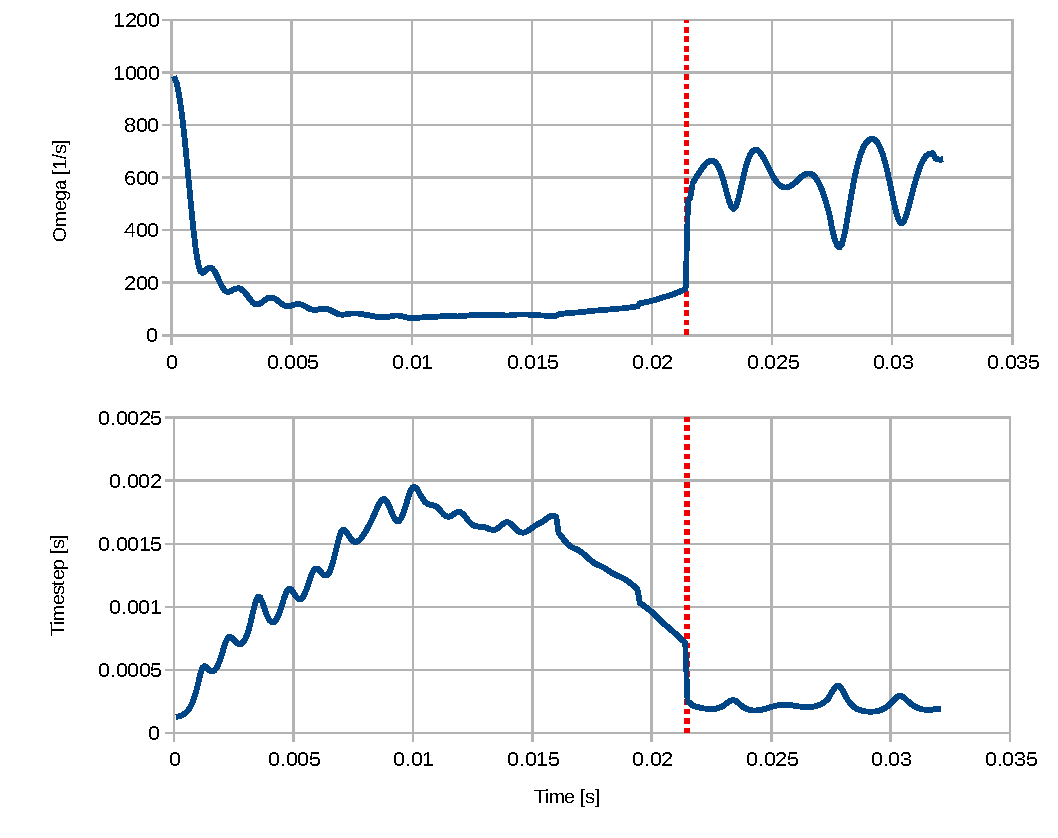
\includegraphics[width=0.8\textwidth]{figures/solution/adaptive-timestep}
\caption{Example for the characteristic frequency~$\omega$ and the associated timestep~$\Delta t^*$ for~$N = 50$. Marked in red is the departure of the arrow.}
\label{fig:adaptive-timestep}
\end{figure}

It can be seen that the characteristic frequency varies greatly over the duration of the simulation, which confirms the usefulness of adaptive time stepping for dynamic bow simulations.
The characteristic frequency is high at the start of the simulation, presumably because the sudden change of releasing the string sends a lot of initial oscillations through the string and the bow limbs.
After this initial disturbance settles down, the motion of the bow turns into a more steady and continuous acceleration of limbs and arrow, represented by a relatively long and smooth section with a low characteristic frequency and larger optimal time steps.
The second spike in characteristic frequency occurs when the string reaches brace height and the arrow separates from the bow, which is not surprising.

Having verified the applicability of the Bergan and Mollestad method for our use case of simulating bows, we still have to define the actual algorithm by which the step size is to be adjusted.
The easiest solution would be to always choose the estimated optimal step size~$\Delta t^*$ as the next step size,

\begin{equation}
\Delta t_{i+1} = \Delta t^*_{i+1}.
\end{equation}

In the original method however, the authors introduce a tuning function~$f$ as

\begin{equation}
\Delta t_{i+1} = f(\xi_{i})\,\Delta t_{i}, \quad \xi_{i} = \frac{\Delta t^*_{i+1}}{\Delta t_{i}}
\end{equation}

in order to moderate the increase or decrease in step size based on the ratio $\xi_{i}$ between the optimal step size and the previously selected step size.
Their proposed tuning function is defined as
%
\begin{align}
f(\xi_{i}) = \begin{cases}
1, & \text{if $\nicefrac{1}{\xi_{p}} < \xi_{i} < \xi_{p}$} \\
2, & \text{if $\xi_{i} > \xi_{m}$} \\
\xi_{i}, & \text{otherwise}
\end{cases}.
\end{align}

Figure \ref{fig:adaptive-timestep-tuning} shows the graph of this function.
It evaluates to~$f(\xi_{i}) = \xi_{i}$ over most of its domain, which means that the suggested timestep is applied, except for the following two modifications:

\begin{itemize}
\item A plateau around~$\xi_{i} = 1$, controlled by the parameter~$\xi_{p}$ with a typical value given as~$1.3$ or~$1.4$.
This plateau prevents the timestep from changing too frequently when the relative changes are only small.
\item A limitation of the increase in step size to a factor of~$\xi_{m}$, typicallay chosen as~$2$.
This prevents the timestep from prematurely increasing too much.
The decrease in step size remains unlimited.
\end{itemize}

\begin{figure}[h]
\centering
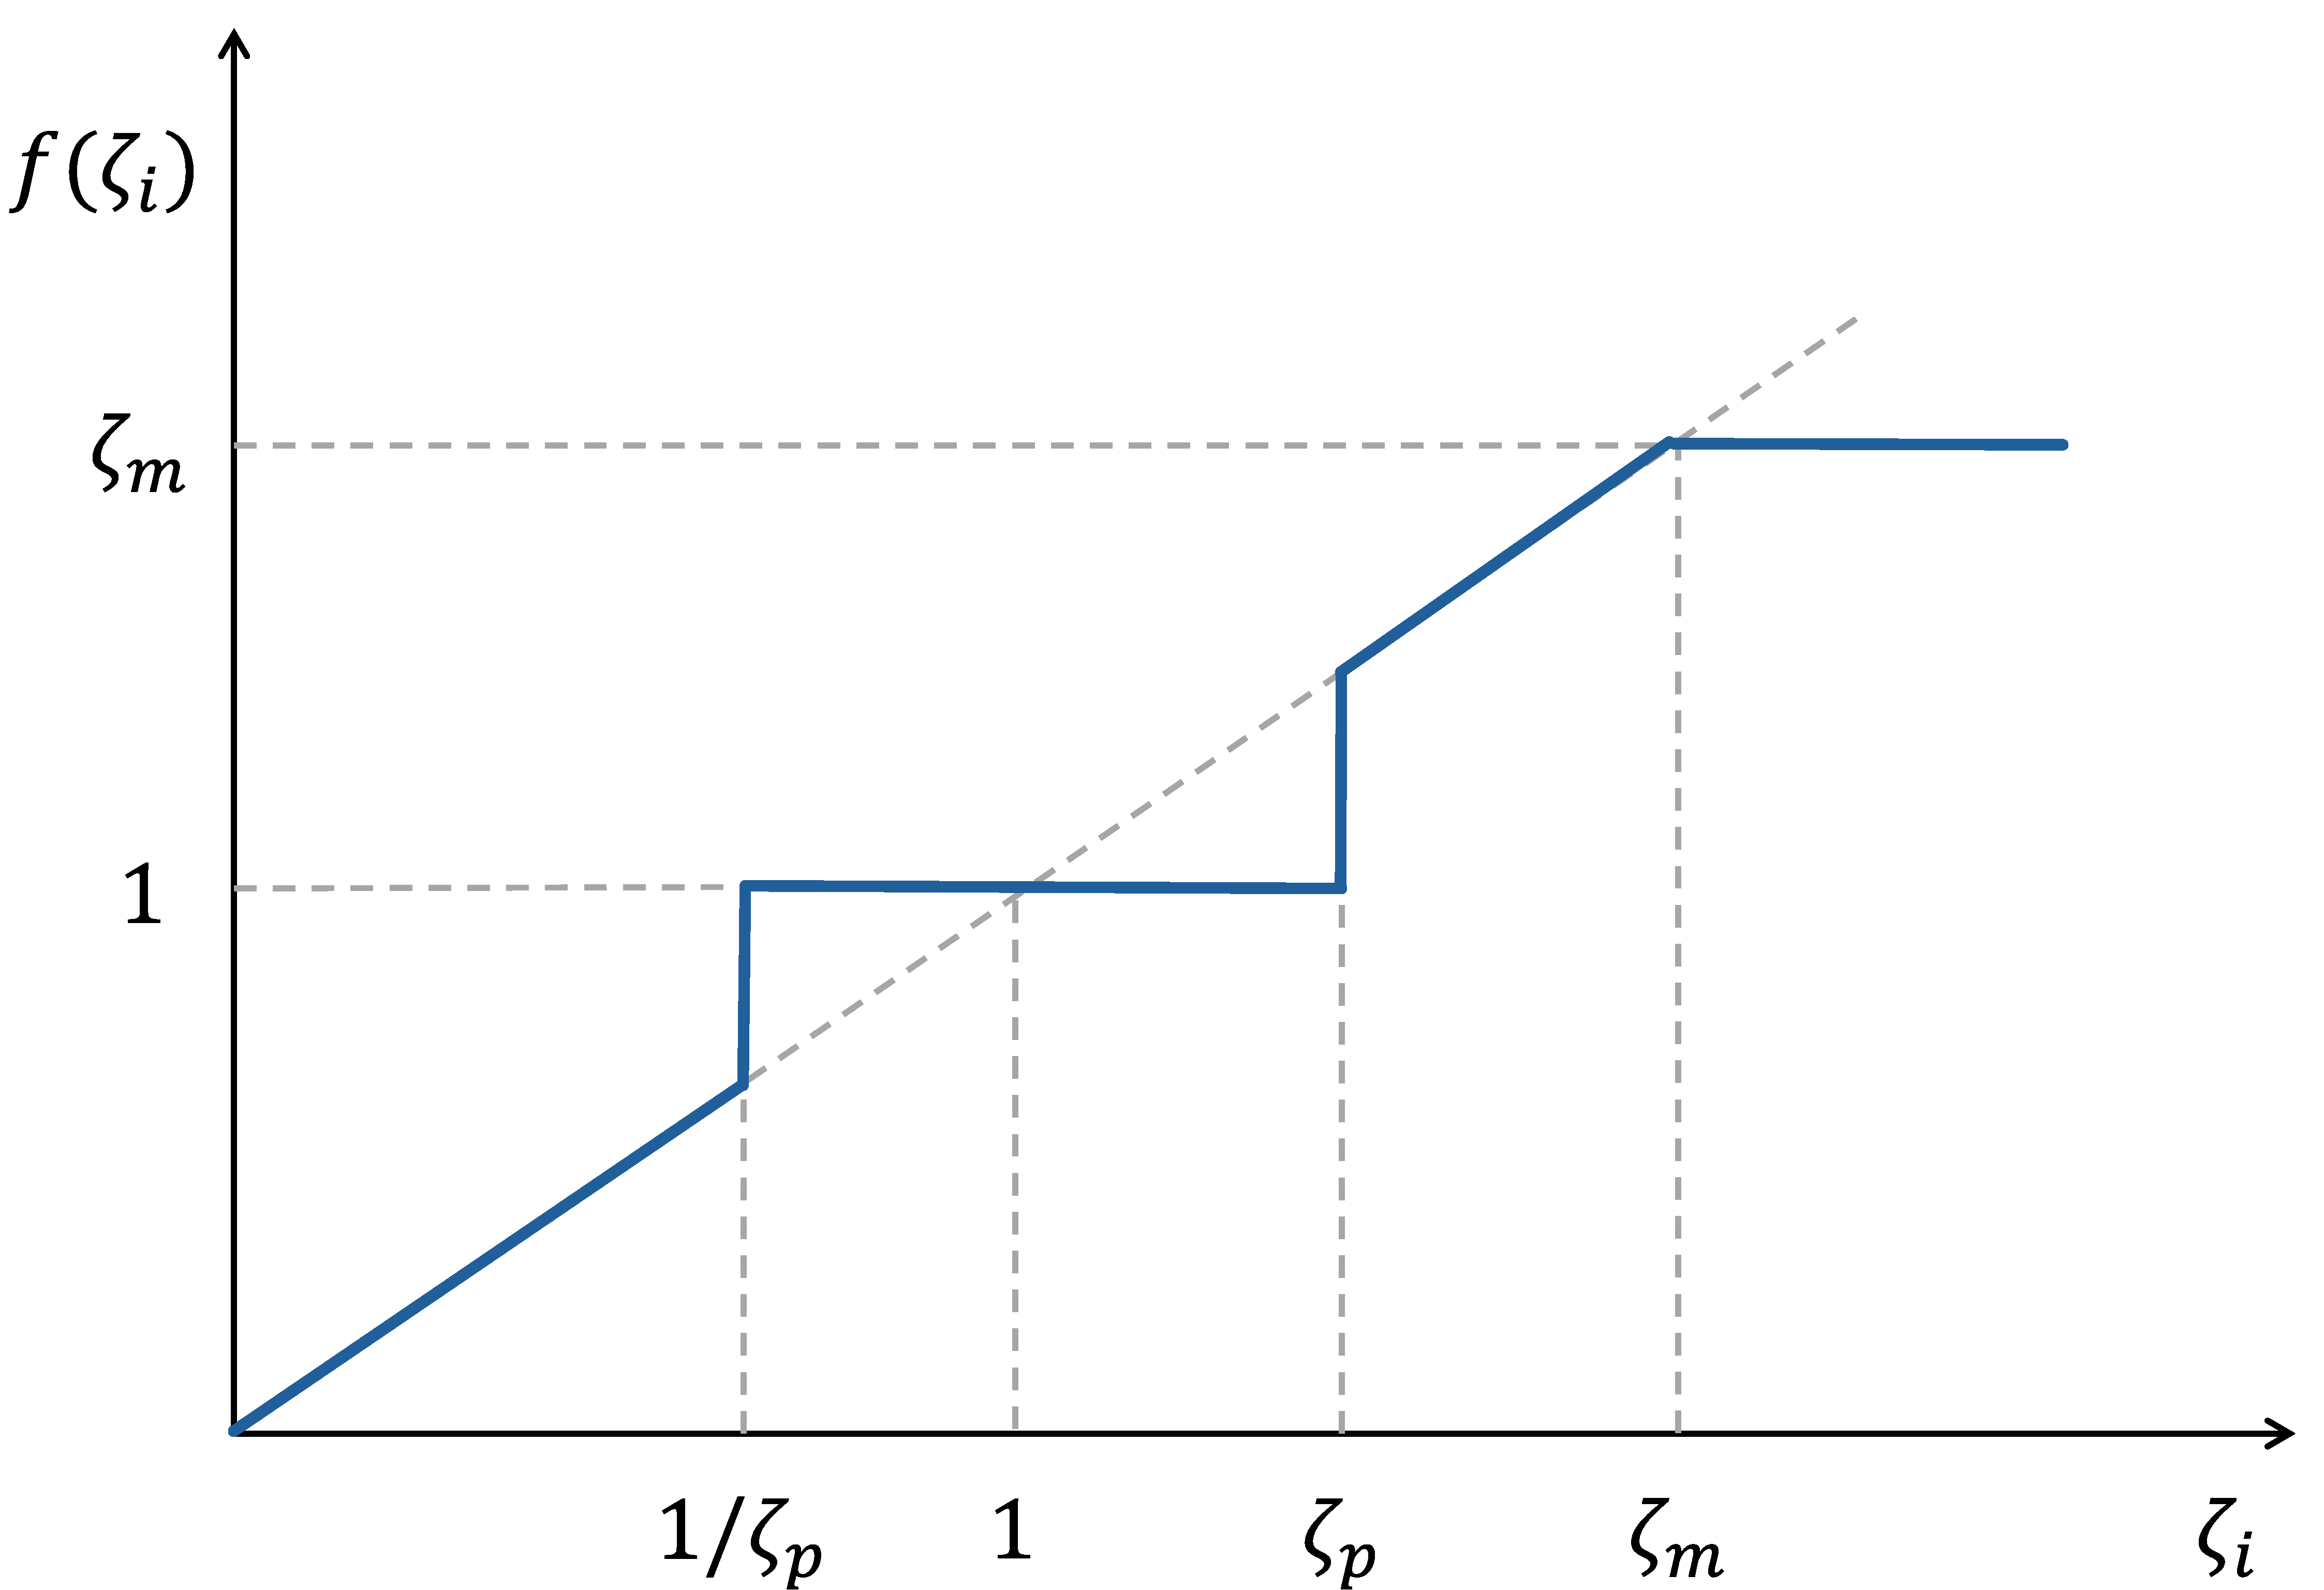
\includegraphics[width=0.6\textwidth]{figures/solution/adaptive-timestep-tuning}
\caption{Tuning function $f(\xi_{i})$ suggested by Bergan and Mollestad}
\label{fig:adaptive-timestep-tuning}
\end{figure}

The reasoning behind the plateau comes from linear dynamic analysis, where changing the timestep causes an additional cost because the system matrices have to be factorized once again.
In nonlinear dynamic analysis this is way less important, since the matrices have to be factorized at each time step anyway due to the equilibrium iterations.
Our implementation therefore does not include this plateau.
The limitation of the relative step size increase has turned out to be essential though.
As another custom modification, we clamp the timestep that results from application of the tuning function between a minimum value $\Delta t_{\min}$ and a maximum value $\Delta t_{\max}$.
The minimum value ensures that the algorithm terminates in a reasonable amount of time and doesn't get stuck in a loop of ever decreasing time steps.
The maximum value ensures a certain minimum time resolution of the solution, even when the integration could have been done with larger time steps.
With these modifications, the actual update logic of the time step used by VirtualBow is given by
%
\begin{align}
f(\xi_{i}) &= \min\Big\{ \xi_{i}, \, 2 \Big\}, \\
\Delta t_{i+1} &= \mathrm{clamp}\Big\{ f(\xi_{i})\cdot\Delta t_{i}, \, \Delta t_{\min}, \, \Delta t_{\max} \Big\}.
\end{align}

The minimum timestep $\Delta t_{\min}$ also serves as the first timestep $\Delta t_{0}$ of the simulation that is needed to start the adaptive scheme.
The value chosen for the first timestep has to be much lower than the expected optimal timestep to ensure that it is too small rather than too large.
An initial timestep that is too small can be increased quickly by the adaptive method in subsequent steps while a timestep that is too large might introduce a permanent error.
The method only ever adaptively changes the next timestep based on the estimated apparent frequency from the previous timestep.
It does not retroactively reject timesteps that were too large, like some more advanced methods do.

\newpage
\section{Stopping event detection and location}

The dynamic simulation in VirtualBow is divided into two sequential phases.
The first phase starts at full draw with the release of the bow string and ends when the arrow has reached the point where it separates from the string and starts flying freely.
After this phase, the simulation model is modified by removing the arrow, which is modelled as a point mass, from the string.
In the second phase the motion of the bow without arrow is then simulated for an additional amount of time in order to capture what happens to the bow after the arrow has left.
This time period is controlled by the "time span factor" in the simulation settings of the software.
The two phases of the dynamic simulation pose different requirements on the dynamic solver when it comes to stopping the simulation.

The second phase is the easier one in this regard.
Here the time integration is to be stopped at a given time~$t = t_\mathrm{end}$.
The only minor complication is that~$t_\mathrm{end}$ does not necessarily line up with the actual time points~$t_{i}$ of the solution and might therefore not be reached exactly.
This is however easily solved by truncating the last timestep accordingly.

The first phase is more complicated since it does not end at a known time.
Instead it ends when a certain event in the solution has occurred, namely the separation of the arrow.
This event is associated with the current accelerations, since the arrow leaves the string as soon as it experiences a negative acceleration that is high enough to overcome the clamping force that holds it on the string.
This event condition can be formulated as

\begin{equation}
e(\boldsymbol{a}) = \boldsymbol{a}[\mathrm{arrow}] + \frac{F_{\mathrm{clamp}}}{m_{\mathrm{arrow}}} = 0 \label{eq:event-function-arrow}
\end{equation}

with $e(\boldsymbol{a})$ being an event function that takes in the current state of the system (in our case only the accelerations are needed) and returns zero when the condition for the event is fulfilled.
The first task is to detect the occurrence of this event while stepping through the numerical solution process.
We assume that an event has occurred between times~$t_{i}$ and~$t_{i+1}$ if there was a sign change of the event function,

\begin{equation}
\sgn\left\{ e(\boldsymbol{a}_{i}) \right\} \neq \sgn\left\{ e(\boldsymbol{a}_{i+1}) \right\}.
\end{equation}

Technically speaking, any odd number of events could have occurred during that timestep, not only one.
Conversely, intervals with no sign change could technically contain any even number of events that go undetected with this approach.
None of that is practically relevant for our bow simulation though since the timesteps are usually small enough to make multiple events very unlikely.
Events can further be narrowed down by only looking for positive or negative sign changes.
In the case of arrow separation (\ref{eq:event-function-arrow}) for example, we are looking for a negative sign change (from positive to negative).

When an event that should stop the simulation is detected between~$t_{i}$ and~$t_{i+1}$, we know that the last time step was actually too large.
If we were being sloppy, we could just stop the simulation at $t_{i+1}$, perform the arrow separation and accept the imperfection that the separation event actually occurred slightly earlier.
This is exactly what VirtualBow did when still using an explicit solution method for the dynamic analysis.
The much smaller timesteps compared to implicit methods made this possible without being to inaccurate.
But by looking back at figure \ref{fig:adaptive-timestep} we can see that this approach would lead to large errors when using the Newmark method, since the timesteps can be far too large.

We therefore have to go the long route and do something more accurate.
The overshooting time point~$t_{i+1}$ is therefore discarded and we restart at~$t_{i}$, this time trying to find a new timestep such that the event occurs exactly at the end of the interval.
This is done by treating the timestep as an additional unknown in the Newmark iterations.
The equilibrium equation (\ref{eq:newmark-residual}) for finding the accelerations at the end of the time interval therefore becomes

\begin{equation}
\boldsymbol{R}(\boldsymbol{a}_{i+1},\,\Delta t) = \boldsymbol{0}. \label{eq:event-location-equation}
\end{equation}

Introducing the additional unknown $\Delta t$ requires us to add an equation as well.
This additional equation or constraint is given by the requirement that the event takes place at $t_{i+1}$, which means that the event function (\ref{eq:event-function-arrow}) must be zero there,

\begin{equation}
e(\boldsymbol{a}_{i+1}) = 0. \label{eq:event-location-constraint}
\end{equation}

So the final task is to solve equation (\ref{eq:event-location-equation}) with the scalar constraint (\ref{eq:event-location-constraint}), which yields both the accelerations $\boldsymbol{a}_{i+1}$ and the correct timestep $\Delta t$.
If this problem seems familiar, it's because it is mathematically equivalent to the problem of displacement control in static analysis, where the static equilibrium equations are solved under the constraint that one of the displacements must match a prescribed value.
We can therefore apply the same numerical method here, namely the constrained Newton-Raphson method, which was outlined in section \ref{sec:constrained-newton-raphson}.

The partial derivative of the residual forces with respect to the step size, which is required for this, is obtained as
%
\begin{align}
\frac{\partial \boldsymbol{R}}{\partial \Delta t} = \frac{\partial \boldsymbol{Q}_{n+1}}{\partial \boldsymbol{u}_{n+1}}\frac{\partial \boldsymbol{u}_{n+1}}{\partial \Delta t} + \frac{\partial \boldsymbol{Q}_{n+1}}{\partial \boldsymbol{\mathrm{v}}_{n+1}}\frac{\partial \boldsymbol{\mathrm{v}}_{n+1}}{\partial \Delta t} &= \boldsymbol{K}_{n+1}\left(\boldsymbol{\mathrm{v}}_{n} + 2\Delta t\left(\left(\nicefrac{1}{2} - \beta\right)\boldsymbol{a}_{n} + \beta \boldsymbol{a}_{n+1}\right) \right) \notag \\
&+ \boldsymbol{D}_{n+1}\left((1 - \gamma)\boldsymbol{a}_{n} + \gamma\boldsymbol{a}_{n+1}\right)
\end{align}

and the partial derivatives of the event function are
%
\begin{equation}
\frac{\partial e}{\partial\boldsymbol{a}_{i+1}} = \boldsymbol{e}_{\mathrm{arrow}}, \quad \frac{\partial e}{\partial\Delta t} = 0
\end{equation}

where $\boldsymbol{e}_{\mathrm{arrow}}$ is the unit vector in the direction that represents the arrow's motion.

\newpage
\subsection{Stopping Criterion and Progress Estimation}

The dynamic simulation is carried out until some stopping criterion is satisfied.
This criterion has to be chosen such that the simulated time interval contains all the information needed by the users while also keeping it as short as possible.
It has to include the separation of the arrow from the string plus some additional time, because some things like e.g. the maximum force on the string tend to happen only after the arrow left the bow.
A related requirement for the stopping criterion is that it must allow estimating the simulation progress, so that it can be shown to the user.

The simplest solution would be to simulate until a fixed time is reached.
This makes the progress estimation very easy, but it also has some drawbacks.
It would require users to specify the simulation time, which can only be found by trial and error and might have to be adjusted for different bows.

The current approach is to simulate a time interval of~$[0,\,\alpha\,T]$ where~$T$ is the (yet unknown) time for the arrow to reach brace height and~$\alpha$ is an arbitrary positive factor.
The default value is~$\alpha = 1.5$. The simulation progress at time~$t$ can now be formally written as

\begin{equation}
\mathrm{progress} = \frac{t}{\alpha\,T} \label{eq:solution:progress}
\end{equation}

i.e. the fraction of simulated time to the total amount of time.
But only formally, because~$T$ is unknown as long as~$t < T$, i.e. as long as the arrow has not yet actually reached brace height.
For this first part of the simulation,~$T$ is estimated by using the current time~$t$ and position~$u$ of the arrow and extrapolate to the time when the arrow is projected to reach brace height.

\begin{figure}[h]
\centering
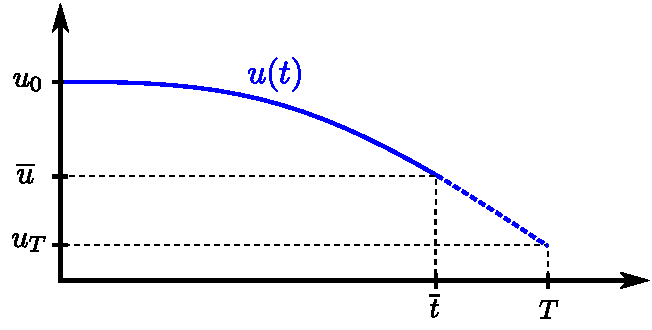
\includegraphics[width=0.6\textwidth]{figures/solution/dynamic-progress}
\caption{Arrow position $u(t)$ during the shot}
\label{fig:solution:dynamic-progress}
\end{figure}

The progression of the arrow position, denoted by~$u(t)$, typically looks somewhat like figure~\ref{fig:solution:dynamic-progress}.
It starts at time~$t = 0$ at full draw~$u_0$ with zero velocity, then increasingly accelerates and reaches brace height~$u_T$ at the time~$t = T$ by definition.
If the acceleration of the arrow is assumed to depend approximately linearly on the distance to brace height (linear force draw curve), then~$u(t)$ will resemble the cosine quarter-wave

\begin{equation}
u(t) \approx \left(u_{0} - u_{T}\right)\cos{\left(C\,t\right)} + u_{T} \label{eq:solution:progress:ansatz}
\end{equation}

with the constant~$C$ that is yet to be determined.
This is of course only a very crude approximation, but it is good enough for estimating the simulation progress.
If we know the current time $t$ and position $u$, we can rearrange equation~(\ref{eq:solution:progress:ansatz}) to get a current value for the constant $C$,

\begin{equation}
C = \frac{1}{t}\,\arccos{\left(\frac{u - u_{T}}{u_{0} - u_{T}}\right)}. \label{eq:solution:progress:constant}
\end{equation}

Knowing~$C$, the time~$T$ can be extrapolated from~(\ref{eq:solution:progress:ansatz}) using the condition~$u(T) = u_{T}$,

\begin{equation}
T = \frac{\pi}{2C} = \frac{\pi}{2}\,t\cdot\arccos\left(\frac{u - u_{T}}{u_{0} - u_{T}}\right)^{-1}.
\end{equation}

Inserting this estimate for $T$ into~(\ref{eq:solution:progress}) results in the final expression for the estimated progress,

\begin{equation}
\mathrm{progress} = \frac{2}{\alpha}\arccos\left(\frac{u - u_{T}}{u_{0} - u_{T}}\right).
\end{equation}

This estimate is used until the arrow has reached brace height.
Then the actual value for~$T$ is known and used within~(\ref{eq:solution:progress}) for the rest of the simulation.
A numerical example for the simulation progress over time is shown in figure \ref{fig:solution:dynamic-progress-estimated}.
The resulting curve is very close to a straight line here, which means that the progress corresponds very well to the simulation time, which is exactly what we want.

\begin{figure}[h]
\centering
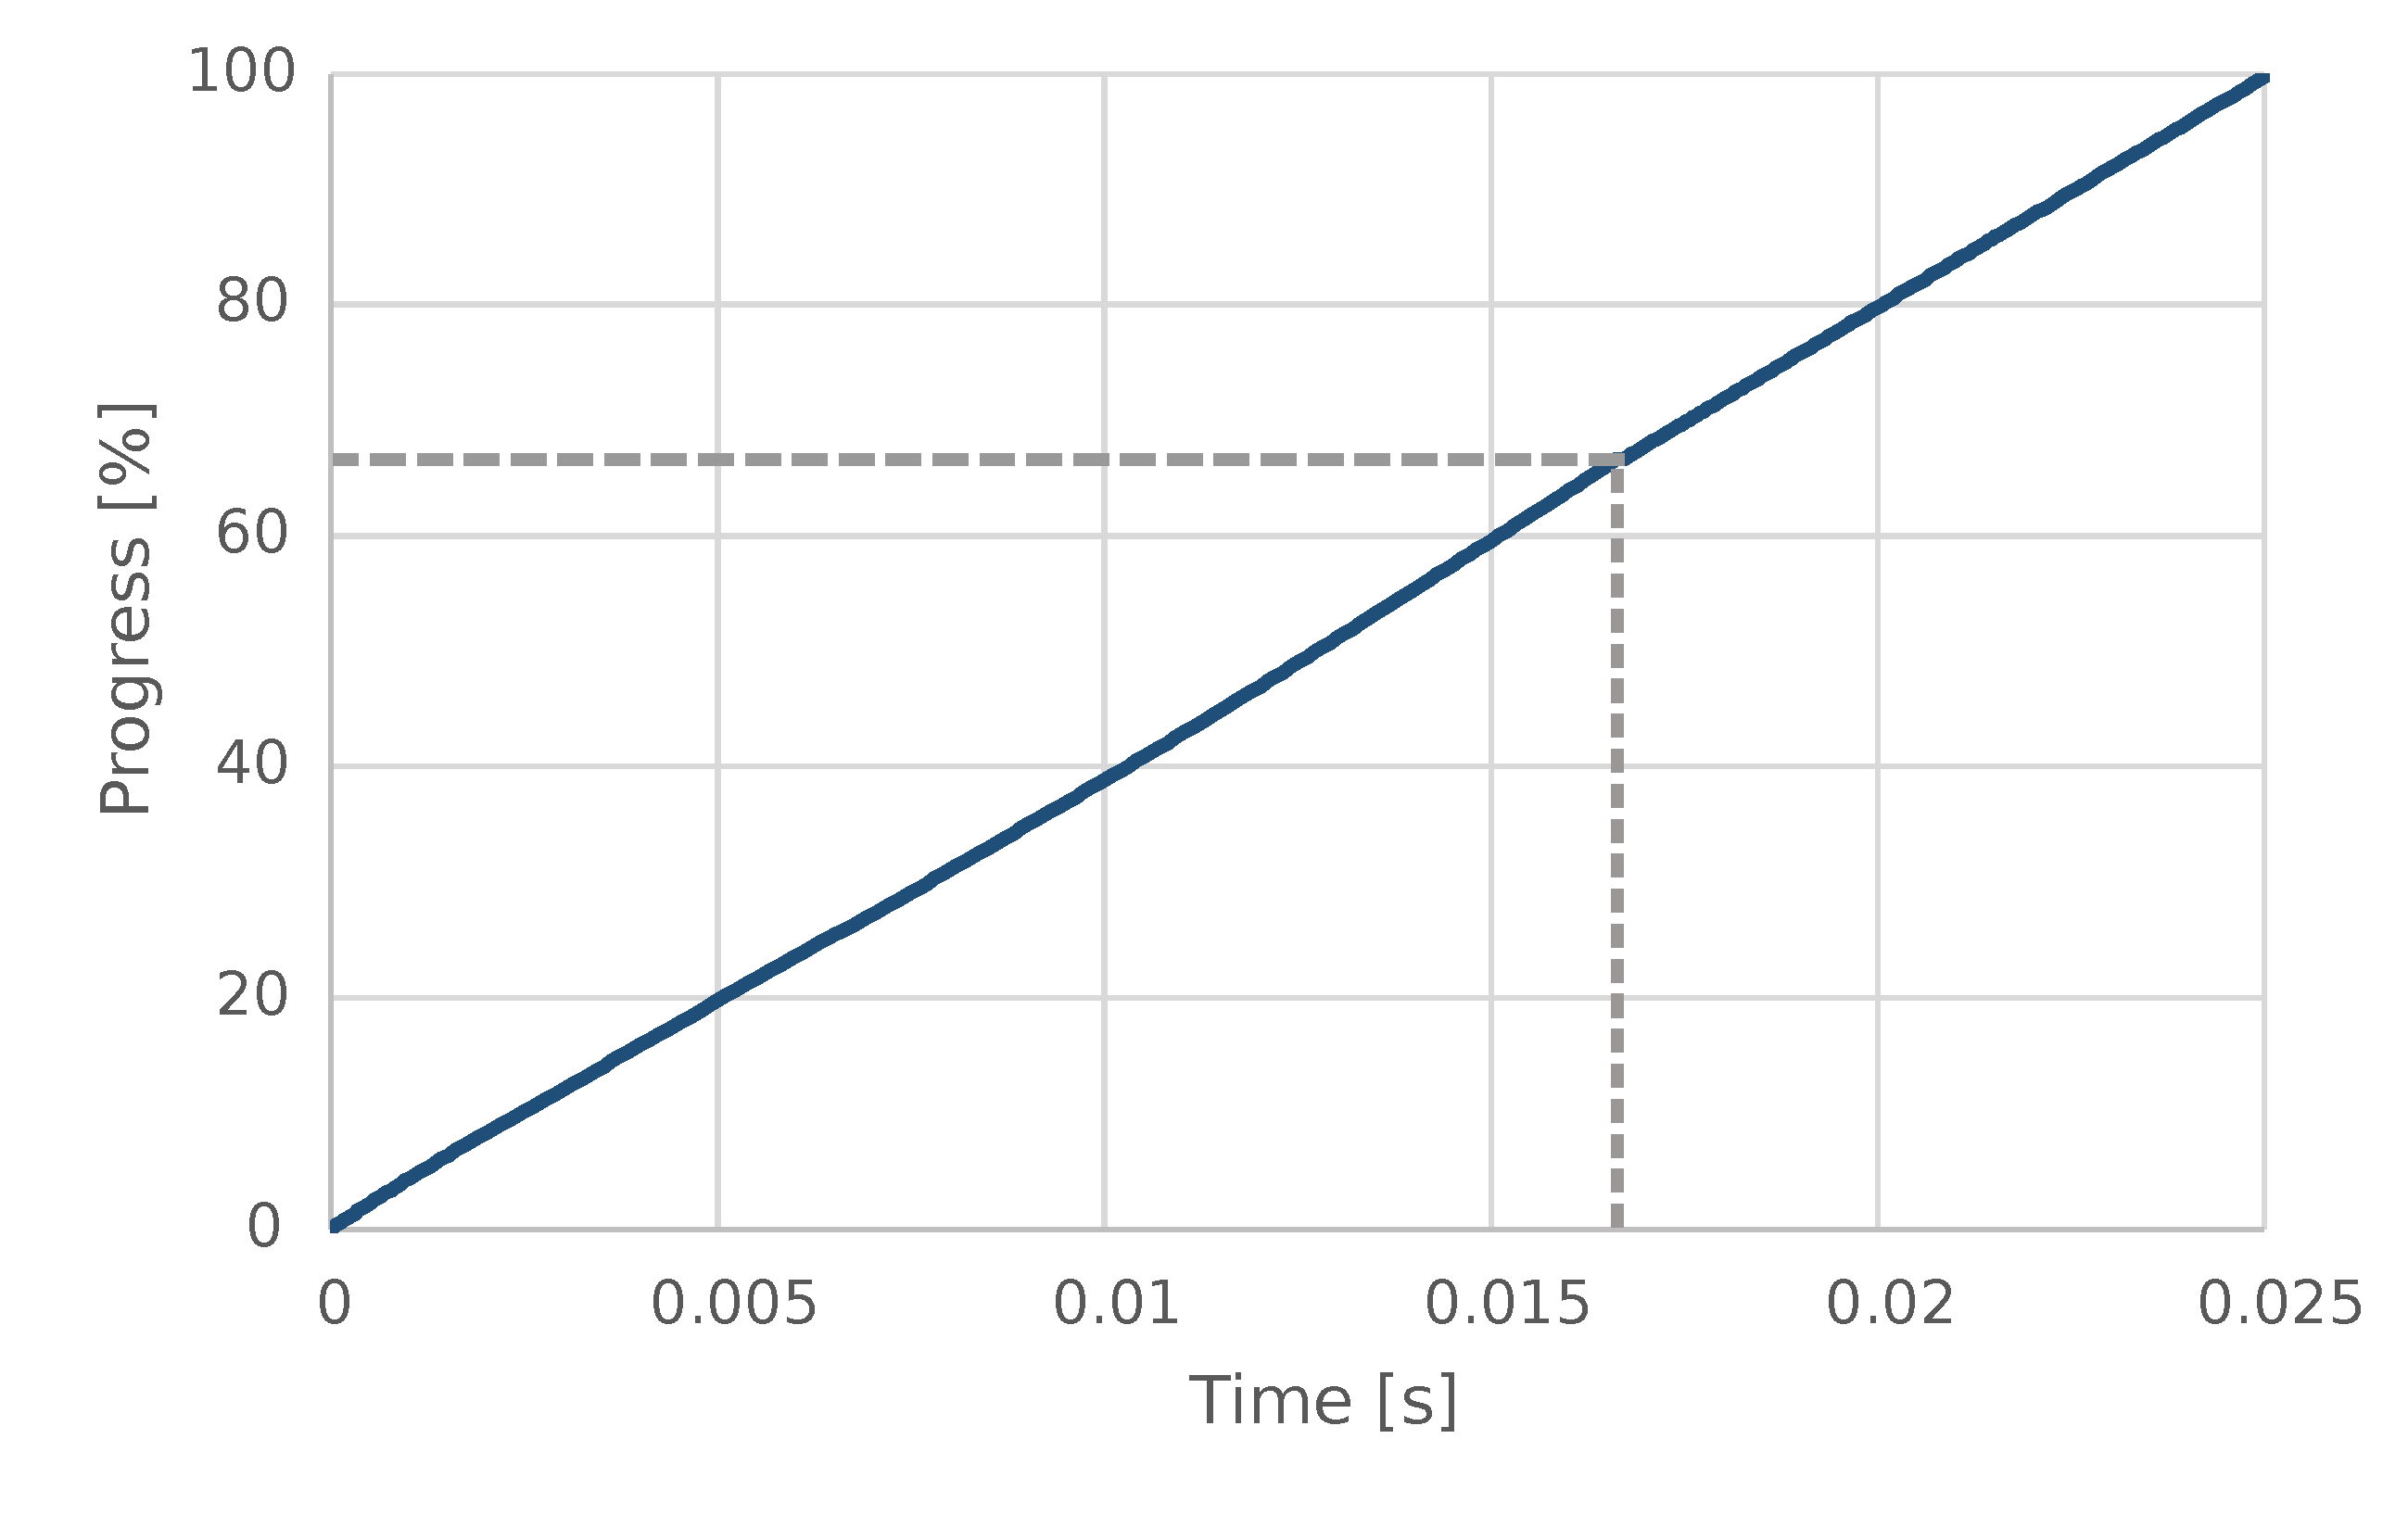
\includegraphics[width=0.6\textwidth]{figures/solution/dynamic-progress-estimated}
\caption{Example for the Simulation progress over time. Marked in grey is the point where the brace height has been reached.}
\label{fig:solution:dynamic-progress-estimated}
\end{figure}